%!TEX root = ../report.tex
%%%%%%%%%%%%%%%%%%%%%%%%%%%%%%%%%%%%%%%%%%%%%%%%%%%%%%%%%%%%%%%%%%%%%%%
%%%%%%%%%%%%%%%%%%%%%%%%%%%%%%%%%%%%%%%%%%%%%%%%%%%%%%%%%%%%%%%%%%%%%%%
%%%%%                                                                 %
%%%%%     z_03_datasheet.                                             %
%%%%%                                                                 %
%%%%% Author:      Florian Zaruba                                     %
%%%%% Created:     13.12.2015                                         %
%%%%% Description: <description>                                      %
%%%%%                                                                 %
%%%%%%%%%%%%%%%%%%%%%%%%%%%%%%%%%%%%%%%%%%%%%%%%%%%%%%%%%%%%%%%%%%%%%%%
%%%%%%%%%%%%%%%%%%%%%%%%%%%%%%%%%%%%%%%%%%%%%%%%%%%%%%%%%%%%%%%%%%%%%%%

\chapter{ASIC Datasheet (Imperio)}

% If you have designed an \gls{asic} during your work, you should
% include a datasheet for your chip into the report. As soon as you
% start testing your fabricated chip, you will be glad to have such a
% datasheet. An example structure of such a datasheet is given in the
% following. For more inspirations on what you may include in your
% datasheet, have a look at the datasheet of a commercial \gls{ic}.

\minitoc

\section{Features}

\begin{itemize}
  \item RISC-V 32-bit architecture.
  \begin{itemize}
    \item 31 x 32-bit General Purpose Registers
    \item Support for RV32C and partial support for M standard extension
    \item Support for hardware loops, post incremental load and stores and SIMD packed instructions
  \end{itemize}
  \item 64 kByte RAM (32 KByte Data and Instruction)
  \item 2 kByte boot ROM
  \item Integrated FLL that offers variable speed from 0-1.2 GHz
  \item JTAG Debug Interface
  \item 19 GPIOs
  \item Peripheral Features
    \begin{itemize}
      \item Two 32-bit counter
      \item UART
      \item I2C
      \item SPI Master
      \item SPI Slave
    \end{itemize}
  \item Full scan-able design with 7 scan chains.
\end{itemize}

%\section{Applications}


\section{Description}

\textbf{Imperio} is the ASIC implementation of PULPino using a RISC-V core. A high-level block diagram can be seen in figure~\ref{fig:block_diagram}. The final mission (once the chip passed testing) of the ASIC is to be employed on a PCB. It therefore was mission critical to have an efficient way of generating the (high) clock, this is achieved by an on-chip FLL. Two 32 kByte on-chip RAMs supply the core with data and instructions. A boot ROM loads the necessary data (through SPI) from an off-chip memory at startup.

\section{Packaging}

A QFN40 package is used with 6 power pins.

\section{Bonding Diagram}

The extended power (ep) bonding is used for this chip. The clock pin is placed on the recommended position in order to facilitate the already manufactured tester boards in use at IIS.

\begin{figure}[htbp]
  \centering 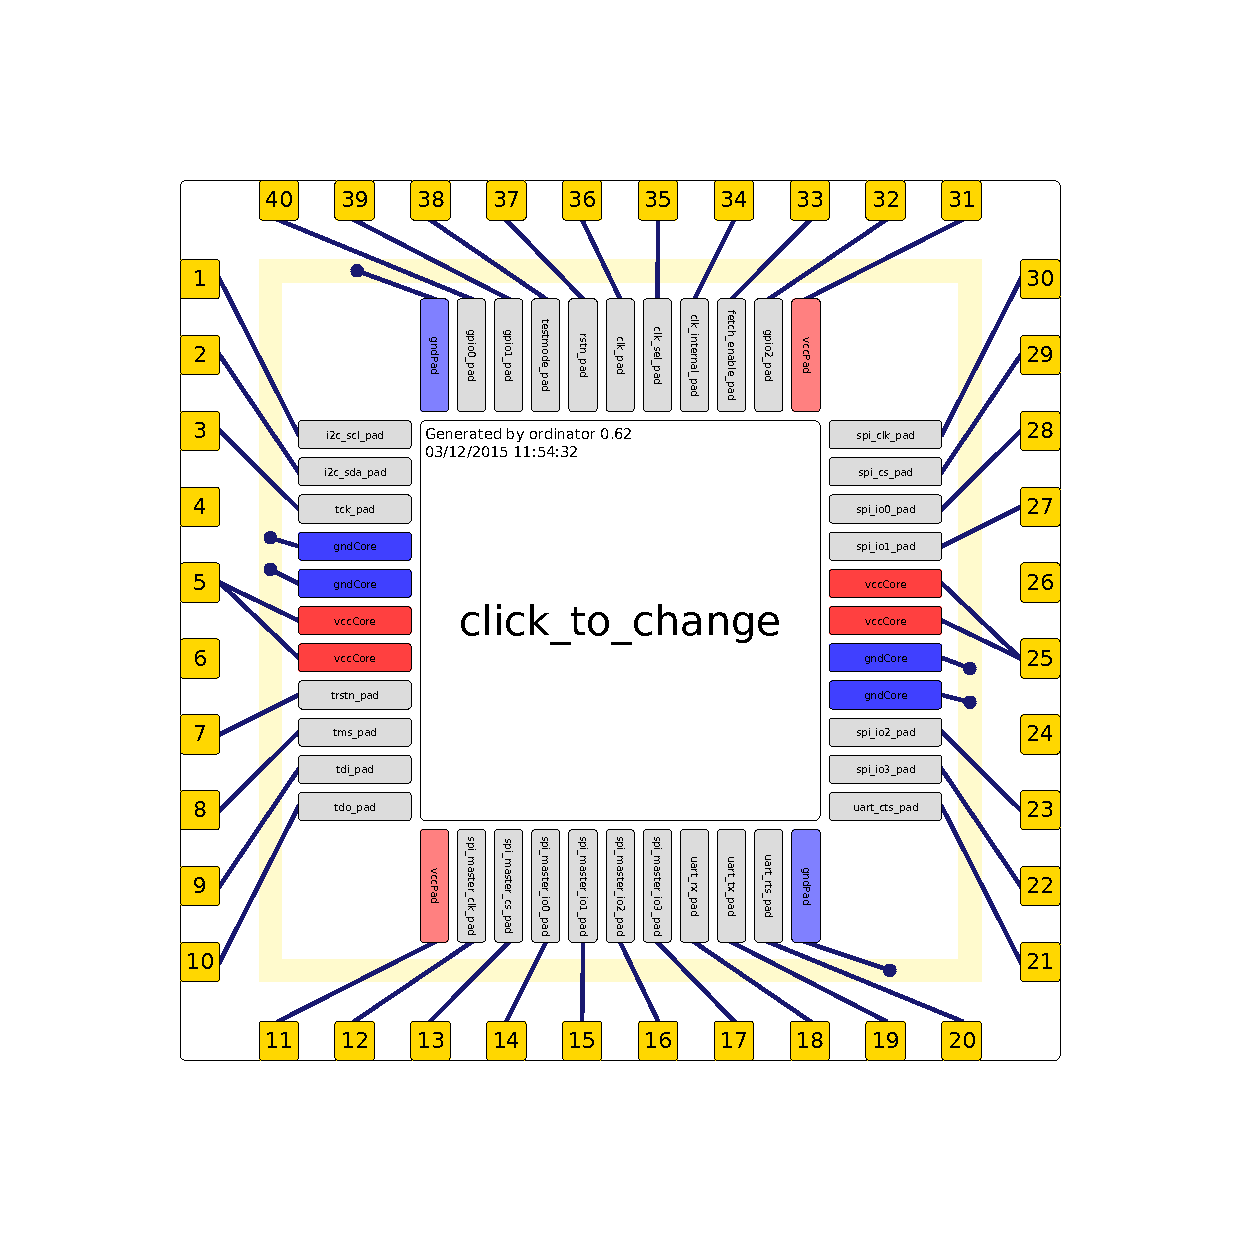
\includegraphics[width=\textwidth]{./figures/pad_instaces_img_ord}
  \caption{Bonding diagram.}
\end{figure}

\section{Pin Map}

\begin{figure}[htbp]
  \centering 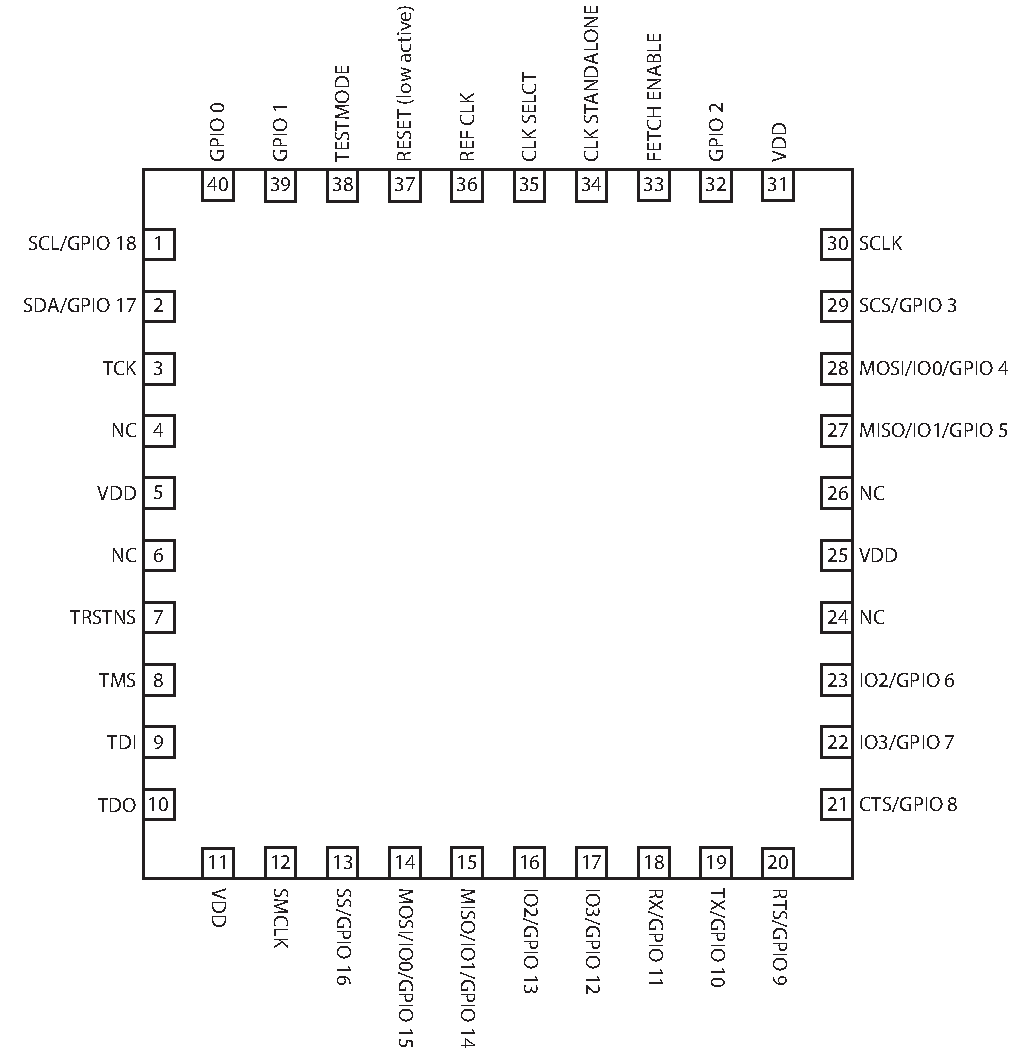
\includegraphics[width=\textwidth]{./figures/pinout_imperio}
  \caption{Imperio pinout (QFN40)}
\end{figure}

\section{Pin Description}
Table~\ref{tab:pins} lists all pins along with their usage, second and testmode function. Testmode is achieved by pulling the \verb+pad_testmode_i+ (38) pin high. Secondary function can be configured by writing the corresponding register in the \pulpino APB peripheral, see~\ref{subsec:pulpino_peripheral}.
\begin{table}[htbp]
 \caption{Pin Description. (Power, IO, Clock, Reset, Test)}
 \label{tab:pins}
\begin{tabular}{|l|l|l|l|l|}
  \hline
  \textbf{Pin No.} & \textbf{Pin Name} & \textbf{Primary function}& \textbf{Sec. Func.}& \textbf{Testmode}\\ \hline
  5, 25 & & \multicolumn{2}{l}{VDD Core} &\\ \hline
  11, 31 & & \multicolumn{2}{l}{VDD Pad} & \\ \hline
  1 & pad\_scl\_io & I2C SCL & GPIO 18  & - \\ \hline
  2 & pad\_sda\_io & I2C SDA & GPIO 17  & - \\ \hline
  3 & pad\_tck\_i & TCK (JTAG) & -  & Scan Clk \\ \hline
  7 & pad\_trstn\_i & TRSTN (JTAG)& -  & Test RST\\ \hline
  8 & pad\_tms\_i & TMS (JTAG) & -  & SI 7 \\ \hline
  9 & pad\_tdi\_i & TDI (JTAG) & -  & - \\ \hline
  10 & pad\_tdo\_o & TDO (JTAG) SCL & -  & SO 7 \\ \hline
  12 & pad\_msclk\_o & SPI Master Clock & -  & - \\ \hline
  13 & pad\_mcs\_io & SPI Master SS & GPIO 16  & SO 5 \\ \hline
  14 & pad\_mio0\_io & SPI Master MOSI/IO0 & GPIO 15  & SO 4 \\ \hline
  15 & pad\_mio1\_io & SPI Master MISO/IO1 & GPIO 14  & SI 4 \\ \hline
  16 & pad\_mio2\_io & SPI Master IO2 & GPIO 13  & SI 5 \\ \hline
  17 & pad\_mio3\_io & SPI Master IO3 & GPIO 12  & - \\ \hline
  18 & pad\_rx\_i & UART RX & GPIO 11  & - \\ \hline
  19 & pad\_tx\_o & UART TX & GPIO 10  & SO 1 \\ \hline
  20 & pad\_rts\_o & UART RTS & GPIO 9  & SO 6 \\ \hline
  21 & pad\_cts\_i & UART CTS & GPIO 8  & SI 6 \\ \hline
  22 & pad\_sio3\_io & SPI Slave IO3 & GPIO 7  & SI 3 \\ \hline
  23 & pad\_sio2\_io & SPI Slave IO2 & GPIO 6  & SO 3 \\ \hline
  27 & pad\_sio1\_io & SPI Slave MISO/IO1 & GPIO 5  & SO 2 \\ \hline
  28 & pad\_sio0\_io & SPI Slave MOSI/IO0 & GPIO 4  & SI 2 \\ \hline
  29 & pad\_scs\_io & SPI Slave CS & GPIO 3  & Scan Clk \\ \hline
  30 & pad\_ssclk\_i & SPI Slave Clock & -  & - \\ \hline
  32 & pad\_gpio\_io[2] & GPIO 2 & -  & - \\ \hline
  33 & pad\_fetch\_enable\_i & fetch enable & -  & - \\ \hline
  34 & pad\_clk\_standalone\_i & Clock Standalone & -  & - \\ \hline
  35 & pad\_clk\_sel\_i & Clock Select & -  & - \\ \hline
  36 & pad\_clk\_i & Clock & -  & Scan Clk \\ \hline
  37 & pad\_rstn\_i & reset (low active) & -  & - \\ \hline
  38 & pad\_testmode\_i & Testmode enable & -  & - \\ \hline
  39 & pad\_gpio\_io[1] & GPIO 1 & - & SI 1 \\ \hline
  40 & pad\_gpio\_io[0] & GPIO 0 & - & Scan En \\ \hline
\end{tabular}  
\end{table}

\section{Floorplan}

The floorplan with macro block positioning is depicted in figure~\ref{fig:floorplan}.

\begin{figure}[h]
  \centering
  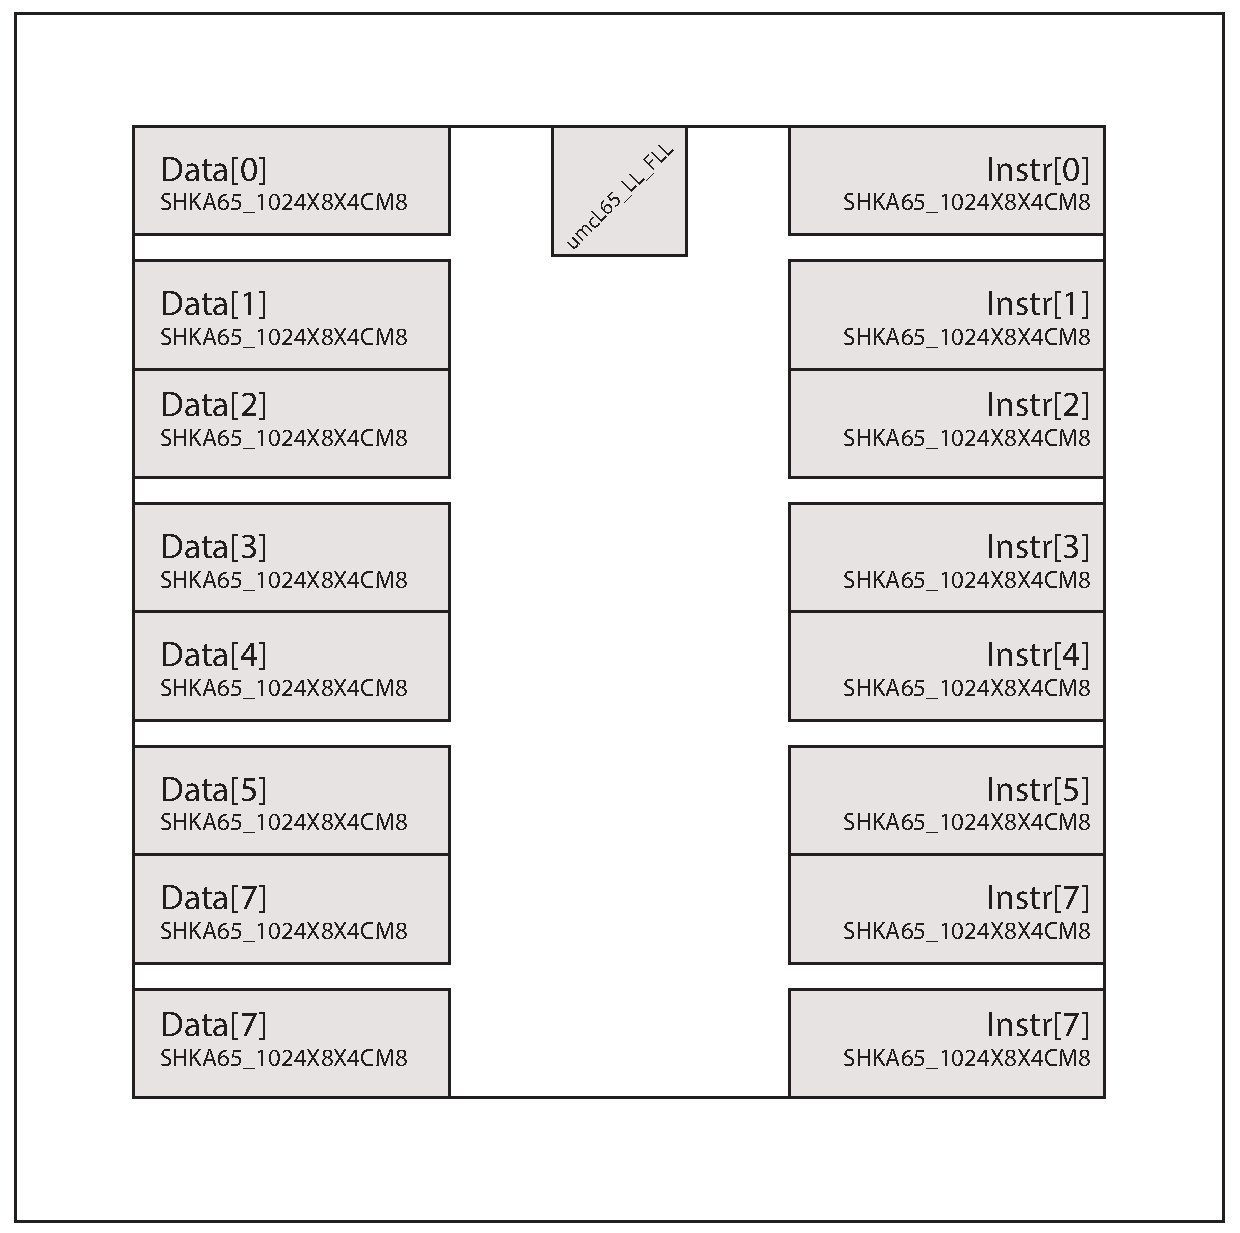
\includegraphics[width=\linewidth]{./figures/floorplan}
  \caption{Floorplan with macro block positioning}
  \label{fig:floorplan}
\end{figure}

\section{Pad Configuration}

\begin{table}[htbp]
 \caption{Pad configuration and corresponding reset values.}
 \label{tab:pads}
\begin{tabularx}{\textwidth}{|X|c|c|c|c|c|c||c|c|c|c|c|c||c|}
  \hline
  \textbf{Pin} & \multicolumn{6}{l||}{\textbf{Primary function}}&  \multicolumn{6}{l||}{\textbf{GPIO}}& \textbf{Test}\\ \hline
    & OE & PD & PU & SMT & SR & DS & OE & PD & PU & SMT & SR & DS & OE \\ \hline
   1  & * & 0 & 0 & 0 & 0 & 0 & 0 & 0 & 0 & 0 & 0 & 0 & 0 \\ \hline
   2  & * & 0 & 0 & 0 & 0 & 0 & 0 & 0 & 0 & 0 & 0 & 0 & 0 \\ \hline
   3  & 0 & 0 & 0 & 0 & 0 & 0 & - & - & - & - & - & - & 0 \\ \hline
   7  & 0 & 0 & 0 & 0 & 0 & 0 & - & - & - & - & - & - & 0 \\ \hline
   8  & 0 & 0 & 0 & 0 & 0 & 0 & - & - & - & - & - & - & 0 \\ \hline
   9  & 0 & 0 & 0 & 0 & 0 & 0 & - & - & - & - & - & - & 0 \\ \hline
   10 & 1 & 0 & 0 & 0 & 0 & 0 & - & - & - & - & - & - & 1 \\ \hline
   12 & 0 & 0 & 0 & 0 & 0 & 0 & - & - & - & - & - & - & 0 \\ \hline
   13 & 1 & 0 & 0 & 0 & 0 & 0 & 0 & 0 & 0 & 0 & 0 & 0 & 1 \\ \hline
   14 & * & 0 & 0 & 0 & 0 & 0 & 0 & 0 & 0 & 0 & 0 & 0 & 1 \\ \hline
   15 & * & 0 & 0 & 0 & 0 & 0 & 0 & 0 & 0 & 0 & 0 & 0 & 0 \\ \hline
   16 & * & 0 & 0 & 0 & 0 & 0 & 0 & 0 & 0 & 0 & 0 & 0 & 0 \\ \hline
   17 & * & 0 & 0 & 0 & 0 & 0 & 0 & 0 & 0 & 0 & 0 & 0 & 0 \\ \hline
   18 & 0 & 0 & 0 & 0 & 0 & 0 & 0 & 0 & 0 & 0 & 0 & 0 & 0 \\ \hline
   19 & 1 & 0 & 0 & 0 & 0 & 0 & 0 & 0 & 0 & 0 & 0 & 0 & 1 \\ \hline
   20 & 0 & 0 & 0 & 0 & 0 & 0 & 0 & 0 & 0 & 0 & 0 & 0 & 1 \\ \hline
   21 & 1 & 0 & 0 & 0 & 0 & 0 & 0 & 0 & 0 & 0 & 0 & 0 & 0 \\ \hline
   22 & * & 0 & 0 & 0 & 0 & 0 & 0 & 0 & 0 & 0 & 0 & 0 & 0 \\ \hline
   23 & * & 0 & 0 & 0 & 0 & 0 & 0 & 0 & 0 & 0 & 0 & 0 & 1 \\ \hline
   27 & * & 0 & 0 & 0 & 0 & 0 & 0 & 0 & 0 & 0 & 0 & 0 & 1 \\ \hline
   28 & * & 0 & 0 & 0 & 0 & 0 & 0 & 0 & 0 & 0 & 0 & 0 & 0 \\ \hline
   29 & 0 & 0 & 0 & 0 & 0 & 0 & 0 & 0 & 0 & 0 & 0 & 0 & 0 \\ \hline
   30 & 0 & 0 & 0 & 0 & 0 & 0 & - & - & - & - & - & - & 0 \\ \hline
   32 & * & 0 & 0 & 0 & 0 & 0 & - & - & - & - & - & - & 0 \\ \hline
   33 & 0 & 0 & 0 & 0 & 0 & 0 & - & - & - & - & - & - & 0 \\ \hline
   34 & 0 & 0 & 0 & 0 & 0 & 0 & - & - & - & - & - & - & 0 \\ \hline
   35 & 0 & 0 & 0 & 0 & 0 & 0 & - & - & - & - & - & - & 0 \\ \hline
   36 & 0 & 0 & 0 & 0 & 0 & 0 & - & - & - & - & - & - & 0 \\ \hline
   37 & 0 & 0 & 0 & 0 & 0 & 0 & - & - & - & - & - & - & 0 \\ \hline
   38 & 0 & 0 & 0 & 0 & 0 & 0 & - & - & - & - & - & - & 0 \\ \hline
   39 & 0 & 0 & 0 & 0 & 0 & 0 & - & - & - & - & - & - & 0 \\ \hline
   40 & 0 & 0 & 0 & 0 & 0 & 0 & - & - & - & - & - & - & 0 \\ \hline
\end{tabularx}  
\end{table}

\section{Interface Description}

\section{Register Map}

\section{Operation Modes}
Imperio distinct functional and test mode. Testmode is achieved by asserting pin \verb+pad_testmode_i+ (38).
\subsection{Functional Modes}
  In functional mode most of the pads serve either as specialized I/O or as GPIO, see table~\ref{tab:pins} for details on the pin configuration.

\subsection{Test Modes}
  When the chip is put into testmode the pads are configured according to table~\ref{tab:pins}. Especially the output enable signals of the pad are configured accordingly, so that all Scan Ins and the Scan Enable signal are inputs and the Scan Outs are configured as outputs. All clock gates are disabled. 

  A special remark on the \verb+pad_fetch_enable_i+ pin. The core does not start fetching instructions until the pin gets asserted. This is meant to accurately time the start times of the execution sequence on the tester. For functional mode this pin should be pulled up.

\FloatBarrier

\section{Electrical Specifications}

\begin{table}[htbp]
 \caption[DC characteristics]{DC characteristics \cite{faraday}:} \label{tab:elect_rec}
\centering
\begin{tabularx}{\textwidth}{|l|X|r|r|c|} 
 \hline
  Symbol & Description & Min. & Max. & Unit \\ \hline
  $V_{Il}$ & Input low voltage & - & 0.7 & V \\ \hline
  $V_{Ih}$ & Input high voltage & 1.7 & - & V \\ \hline
  $V_{Ol}$ & Output low voltage & - & 0.4 & V \\ \hline
  $V_{Oh}$ & Output high voltage & 1.85 & - & V \\ \hline
  Pull-up & Pull-up-resistor & 53 & 53 & k $\Omega$ \\ \hline
  Pull-down & Pull-down-resistor & 53 & 53 & k $\Omega$ \\ \hline
  %$I_O$ & Output driving & \multicolumn{2}{r|}{8} & $mA$ \\ \hline
 \end{tabularx}
 \end{table}

\subsection{Recommended Operating Regions}
\begin{table}[htbp]
 \caption[Recommended Operating Conditions]{Recommended Operating Conditions \cite{faraday}}
 \label{tab:elect_rec}
\centering\begin{tabularx}{\textwidth}{|l|X|r|r|r|c|} \hline
Symbol & Description & Min. & Typ. & Max. & Unit \\ \hline
\textit{VDD} & Core power supply & 1.08 & 1.2 & 1.32 & V \\ \hline
\textit{VDDIO} & IO power supply & 2.25 & 2.5 & 2.75 & V \\ \hline
$T_J$ & Operating junction temperature & -40 & 25 & 125 &  $^\circ$C \\ \hline
 \end{tabularx}
 \end{table}

% \subsection{Absolute Maximum Ratings}

%  \begin{table}[ht]
%  \caption[Absolute Maximum Ratings]{Absolute Maximum Ratings \cite{faraday}}
%  \label{tab:elect_rec}
% \centering\begin{tabularx}{\textwidth}{|l|X|c|c|c|} \hline
% Symbol & Description & Rating & Unit \\ \hline
% \textit{VDD} & Core power supply & -0.5 $\sim$ 2.5 & $V$ \\ \hline
% \textit{VDDIO} & Pad power supply & -0.5 $\sim$ 4.6 & $V$ \\ \hline
% $V_{In}$ & Input voltage &  -0.5 $\sim$ 4.6 & $V$ \\ \hline
% $I_{In}$ & DC input current & 50 & $mA$ \\ \hline
% $I_{Out}$ & DC output current & 50 & $mA$ \\ \hline
%  \end{tabularx}
%  \end{table}
